\section{Supplementary Material}

\textbf{Use of LLMs.}
In this paper, LLMs were utilized in two primary ways: (1) as auxiliary tools for data cleaning and preliminary quality checks under human supervision. (2) As evaluation targets in benchmark experiments. To ensure data quality, no content directly generated by LLMs was included in the released dataset. During manuscript preparation, LLMs were employed for minor language polishing. All ideas, methodologies, and conclusions are original contributions of authors.

\subsection{Supplementary Statistics of OmniEduBench}

In Table~\ref{atab:arr_kd}, we present the bilingual names and abbreviations of all subjects in the knowledge dimension. 
In Table~\ref{atab:arr_cd}, we present the bilingual names and abbreviations of all subjects in the cultivation dimension.
In Tables~\ref{atab:sta_k12}, ~\ref{atab:sta_kd_other}, and \ref{atab:sta_cd}, we present the detailed data distribution for all 61 subjects.


\begin{table}[htbp]
    \centering
    \caption{Bilingual names and abbreviations of all subject in the knowledge dimension.}
    \vspace{0.2mm}
    \resizebox{0.99\textwidth}{!}{
    \begin{tabular}{lll}
        \toprule
        \textbf{Abbreviation} & \textbf{English Name} & \textbf{Chinese Name} \\
        \midrule
        MATH & Mathematics & \cc{数学} \\
        CHEM & Chemistry & \cc{化学} \\
        BIO & Biology & \cc{生物} \\
        PHY & Physics & \cc{物理} \\
        NSCI & Nature \& Science & \cc{自然与科学} \\
        PSTAT & Probability \& Statistics & \cc{概率论与数理统计} \\
        PPHY & Plant Physiology & \cc{植物生理学} \\
        CS & Computer Science & \cc{计算机} \\
        BCHEM & Biochemistry & \cc{生物化学} \\
        OS & Operating Systems & \cc{操作系统} \\
        AMATH & Advanced Mathematics & \cc{高等数学} \\
        CNET & Computer Networks & \cc{计算机网络} \\
        LANG & Chinese Language & \cc{语文} \\
        GEO & Geography & \cc{地理} \\
        HIST & History & \cc{历史} \\
        IART & Introduction to Arts & \cc{艺术概论} \\
        ILING & Introduction to Linguistics & \cc{语言学概论} \\
        HSTUD & History Studies / Historiography & \cc{历史学} \\
        HFA & History of Foreign Art & \cc{外国美术简史} \\
        IARCH & Introduction to Archaeology & \cc{考古学概论} \\
        HACL & History of Ancient Chinese Literature & \cc{中国古代文学史} \\
        HWP & History of Western Philosophy & \cc{西方哲学史} \\
        POL & Politics & \cc{政治} \\
        IMOR & Ideology \& Morality & \cc{思想品德} \\
        MGMT & Management & \cc{管理学} \\
        HRM & Human Resource Management & \cc{人力资源管理} \\
        TAX & Taxation & \cc{税收学} \\
        PSCI & Political Science & \cc{政治学} \\
        MARX & Marxist Theory & \cc{马克思主义理论} \\
        ELOG & Economic Logic & \cc{经济学逻辑能力} \\
        NJE & National Judicial Exam & \cc{法考真题} \\
        CLAW & Criminal Law & \cc{刑法学} \\
        CVLAW & Civil Law & \cc{民法学} \\
        LAW & Law / Jurisprudence & \cc{法学} \\
        TCM & Traditional Chinese Medicine & \cc{中医综合} \\
        WMED & Western Medicine & \cc{西医综合} \\
        NURS & Nursing & \cc{护理学} \\
        IT & Information Technology & \cc{信息技术} \\
        CEM & Civil Engineering Materials & \cc{土木工程材料} \\
        EDU & Education & \cc{教育学} \\
        PSY & Psychology & \cc{心理学} \\
        \bottomrule
    \end{tabular}}
    \label{atab:arr_kd}
\end{table}

\begin{table}[htbp]
    \centering
    \caption{Bilingual names and abbreviations of all subject in the cultivation dimension}
    \vspace{0.2mm}
    \resizebox{0.99\textwidth}{!}{
    \begin{tabular}{lll}
        \toprule
        \textbf{Abbreviation} & \textbf{English Meaning} & \textbf{Chinese Name} \\
        \midrule
        \multicolumn{3}{l}{\textit{Major Categories}} \\
        \midrule
        TCS & Thinking \& Cognitive Skills & \cc{思维与认知能力} \\
        EMH & Emotional \& Mental Health & \cc{情感与心理健康} \\
        SIS & Social \& Interpersonal Skills & \cc{社会与人际交往} \\
        CV & Character \& Values & \cc{品格与价值观} \\
        PD & Personalized Development & \cc{个性化发展} \\
        TFS & Teaching Feedback \& Support & \cc{教学反馈与支持} \\
        \midrule
        \multicolumn{3}{l}{\textit{Subcategories}} \\
        \midrule
        IC & Innovation \& Creativity & \cc{创新与创造力} \\
        PSS & Problem-Solving Skills & \cc{问题解决能力} \\
        CT & Critical Thinking & \cc{批判性思维} \\
        GRL & Guided Reflective Learning & \cc{反思性学习引导} \\
        MA & Metacognitive Abilities & \cc{元认知能力} \\
        GKT & Guiding Knowledge Transfer & \cc{引导知识迁移能力} \\
        ER & Emotional Regulation & \cc{情绪调控能力} \\
        EC & Empathy \& Compassion & \cc{同理心与共情} \\
        SCSE & Self-Confidence \& Self-Efficacy & \cc{自信心与自我效能感} \\
        PR & Psychological Resilience & \cc{心理韧性与抗挫力} \\
        GM & Growth Mindset & \cc{成长型思维} \\
        TC & Teamwork \& Collaboration & \cc{团队协作能力} \\
        ECOM & Effective Communication & \cc{有效沟通能力} \\
        SR & Social Responsibility & \cc{社会责任感} \\
        RA & Responsibility \& Accountability & \cc{责任感与担当} \\
        IH & Integrity \& Honesty & \cc{正直与诚信} \\
        PLP & Personalized Learning Paths & \cc{个性化学习路径} \\
        IDL & Interest-Driven Learning & \cc{兴趣驱动学习} \\
        HT & Heuristic Teaching & \cc{启发式教学} \\
        CTF & Constructive \& Timely Feedback & \cc{反馈的建设性与及时性} \\
        \bottomrule
    \end{tabular}}
    \label{atab:arr_cd}
    \vspace{-8mm}
\end{table}

\begin{table}[htbp]
    \centering
    \caption{Statistics of OmniEduBench for K-12 in the knowledge dimension.}
    \vspace{0.2mm}
    \resizebox{0.99\textwidth}{!}{
    \begin{tabular}{ll|ccccc|c}
        \toprule
        \multicolumn{1}{c}{\multirow{2}{*}{\textbf{\begin{tabular}[c]{@{}c@{}}English Name\end{tabular}}}} & 
        \multicolumn{1}{c|}{\multirow{2}{*}{\textbf{Chinese Name}}} 
        & \textbf{\cc{选择题}} & \textbf{\cc{多选题}} & \textbf{\cc{填空题}} & \textbf{\cc{解答题}} & \textbf{\cc{复合题}} & \textbf{\cc{总计}} \\
        & & \begin{tabular}[c]{@{}c@{}}Multiple\\ choice\end{tabular} 
        & \begin{tabular}[c]{@{}c@{}}Multiple\\ answer\end{tabular} 
        & \begin{tabular}[c]{@{}c@{}}Fill-in-\\ the-blank\end{tabular} 
        & \begin{tabular}[c]{@{}c@{}}Short\\ -answer\end{tabular} 
        & \begin{tabular}[c]{@{}c@{}}Composite\\ questions\end{tabular} 
        & Total \\
        \midrule
        Chinese & \textbf{\cc{语文}} & 350 & 8 & 1697 & 1261 & 51 & 3367 \\
        Mathematics & \textbf{\cc{数学}} & 527 & 12 & 1865 & 1181 & 142 & 3727 \\
        Chemistry & \textbf{\cc{化学}} & 274 & 76 & 799 & 477 & 14 & 1640 \\
        History & \textbf{\cc{历史}} & 67 & 24 & 63 & 211 & 5 & 370 \\
        Geography & \textbf{\cc{地理}} & 78 & 31 & 277 & 173 & 4 & 563 \\
        Moral Education & \textbf{\cc{思想品德}} & 14 & 30 & 34 & 56 & 4 & 138 \\
        Politics & \textbf{\cc{政治}} & 260 & 241 & 281 & 64 & 12 & 858 \\
        Physics & \textbf{\cc{物理}} & 82 & 15 & 178 & 46 & 16 & 337 \\
        Biology & \textbf{\cc{生物}} & 115 & 94 & 360 & 124 & 0 & 693 \\
        Nature Science & \textbf{\cc{自然与科学}} & 8 & 0 & 23 & 22 & 0 & 53 \\
        \begin{tabular}[c]{@{}c@{}}Information\\ Technology\end{tabular} & \textbf{\cc{信息技术}} & 18 & 2 & 14 & 1 & 1 & 36 \\
        \midrule
        Total & \textbf{\cc{总计}} & 1793 & 533 & 5591 & 3616 & 249 & 11.782K \\
        \bottomrule
    \end{tabular}}
    \label{atab:sta_k12}
    \vspace{-8mm}
\end{table}

\begin{sidewaystable}[htbp]
    \centering
    \caption{Statistics of OmniEduBench for high, college, and professional schools in the knowledge dimension}
    \vspace{0.2mm}
    \resizebox{0.99\textwidth}{!}{
        \begin{tabular}{ll|cccccccccc|c}
            \toprule
            \multicolumn{1}{c}{\multirow{2}{*}{\textbf{\begin{tabular}[c]{@{}c@{}}English Name\end{tabular}}}} & 
            \multicolumn{1}{c|}{\multirow{2}{*}{\textbf{Chinese Name}}} &
            \textbf{\cc{单选题}} & \textbf{\cc{多选题}} & \textbf{\cc{名词解释}} & \textbf{\cc{简答题}} & \textbf{\cc{论述题}} & \textbf{\cc{案例分析题}} & \textbf{\cc{填空题}} & \textbf{\cc{计算题}} & \textbf{\cc{判断题}} & \textbf{\cc{逻辑推理}} & \textbf{\cc{总计}} \\
            & & \begin{tabular}[c]{@{}c@{}}Single\\ Choice\end{tabular} & 
            \begin{tabular}[c]{@{}c@{}}Multiple\\ choice\end{tabular} &
            \begin{tabular}[c]{@{}c@{}}Term\\ explanation\end{tabular} &
            \begin{tabular}[c]{@{}c@{}}Short\\ answer\end{tabular} &
            Essay &
            \begin{tabular}[c]{@{}c@{}}Case\\ analysis\end{tabular} &
            \begin{tabular}[c]{@{}c@{}}Fill-in-\\ blank\end{tabular} &
            Calculation &
            \begin{tabular}[c]{@{}c@{}}True/\\ False\end{tabular} &
            \begin{tabular}[c]{@{}c@{}}Logical\\ reasoning\end{tabular} &
            Total \\
            \midrule
            Traditional Chinese Medicine & \textbf{\cc{中医综合}} & 230 & 317 & 0 & 0 & 0 & 0 & 0 & 0 & 0 & 0 & 547 \\
            Chinese Ancient Literary History & \textbf{\cc{中国古代文学史}} & 31 & 14 & 20 & 27 & 19 & 0 & 0 & 0 & 0 & 0 & 111 \\
            Human Resource Management & \textbf{\cc{人力资源管理}} & 36 & 35 & 9 & 38 & 19 & 6 & 4 & 0 & 0 & 0 & 147 \\
            Jurisprudence & \textbf{\cc{法学}} & 109 & 153 & 0 & 0 & 0 & 0 & 0 & 0 & 0 & 0 & 262 \\
            Criminal Law & \textbf{\cc{刑法学}} & 158 & 171 & 2 & 3 & 1 & 0 & 0 & 0 & 0 & 0 & 335 \\
            History & \textbf{\cc{历史学}} & 26 & 0 & 68 & 6 & 17 & 12 & 0 & 0 & 0 & 0 & 129 \\
            Civil Engineering Materials & \textbf{\cc{土木工程材料}} & 36 & 2 & 67 & 21 & 57 & 2 & 107 & 39 & 3 & 0 & 334 \\
            A Brief History of Foreign Art & \textbf{\cc{外国美术简史}} & 0 & 0 & 61 & 37 & 15 & 14 & 0 & 0 & 0 & 0 & 127 \\
            Psychology & \textbf{\cc{心理学}} & 146 & 45 & 0 & 35 & 0 & 1 & 0 & 0 & 0 & 0 & 227 \\
            Nursing & \textbf{\cc{护理学}} & 61 & 41 & 0 & 5 & 0 & 16 & 0 & 0 & 0 & 0 & 123 \\
            Operating Systems & \textbf{\cc{操作系统}} & 98 & 0 & 0 & 0 & 0 & 59 & 0 & 0 & 0 & 0 & 157 \\
            Politics & \textbf{\cc{政治}} & 7 & 47 & 0 & 0 & 0 & 36 & 0 & 0 & 0 & 0 & 90 \\
            Pedagogy & \textbf{\cc{教育学}} & 179 & 0 & 0 & 45 & 39 & 0 & 0 & 0 & 14 & 0 & 277 \\
            Advanced Mathematics & \textbf{\cc{高等数学}} & 43 & 0 & 0 & 0 & 3 & 0 & 40 & 55 & 0 & 0 & 141 \\
            Plant Physiology & \textbf{\cc{植物生理学}} & 66 & 0 & 0 & 134 & 33 & 48 & 0 & 0 & 0 & 0 & 281 \\
            Probability and Mathematical Statistics & \textbf{\cc{概率论与数理统计}} & 0 & 0 & 0 & 2 & 0 & 74 & 0 & 257 & 0 & 0 & 333 \\
            Civil Law & \textbf{\cc{民法学}} & 91 & 187 & 0 & 0 & 0 & 0 & 0 & 0 & 0 & 0 & 278 \\
            judicial Practice & \textbf{\cc{法考真题}} & 193 & 430 & 0 & 0 & 0 & 0 & 0 & 0 & 0 & 0 & 623 \\
            Biochemistry\ & \textbf{\cc{高等生物化学}} & 62 & 0 & 0 & 70 & 23 & 0 & 0 & 0 & 0 & 0 & 155 \\
            Taxation & \textbf{\cc{税收学}} & 19 & 2 & 7 & 30 & 0 & 2 & 0 & 23 & 11 & 0 & 94 \\
            Management & \textbf{\cc{管理学}} & 0 & 0 & 0 & 0 & 0 & 0 & 0 & 0 & 0 & 202 & 202 \\
            Economics & \textbf{\cc{经济学逻辑能力}} & 2 & 0 & 0 & 0 & 0 & 0 & 0 & 0 & 0 & 58 & 60 \\
            Archaeology & \textbf{\cc{考古学概论}} & 0 & 0 & 121 & 0 & 0 & 0 & 0 & 0 & 0 & 0 & 121 \\
            Introduction to Archaeology & \textbf{\cc{艺术概论}} & 57 & 43 & 80 & 45 & 26 & 0 & 0 & 0 & 37 & 0 & 288 \\
           Western Medicine & \textbf{\cc{西医综合}} & 159 & 119 & 0 & 0 & 0 & 0 & 0 & 0 & 0 & 0 & 278 \\
            Western Philosophy & \textbf{\cc{西方哲学史}} & 51 & 0 & 0 & 0 & 0 & 0 & 0 & 0 & 0 & 0 & 51 \\
            Computer Science  & \textbf{\cc{计算机}} & 137 & 0 & 0 & 0 & 0 & 47 & 0 & 0 & 0 & 0 & 184 \\
            Computer Networks & \textbf{\cc{计算机网络}} & 91 & 0 & 0 & 0 & 0 & 50 & 0 & 0 & 0 & 0 & 141 \\
            Introduction to Linguistics & \textbf{\cc{语言学概论}} & 53 & 29 & 24 & 22 & 26 & 18 & 0 & 0 & 0 & 0 & 172 \\
            Marxist Theory & \textbf{\cc{马克思主义理论}} & 0 & 0 & 20 & 31 & 13 & 7 & 0 & 0 & 0 & 0 & 71 \\
            \midrule
            Total & \textbf{\cc{总计}} & 2141 & 1635 & 479 & 551 & 291 & 392 & 151 & 374 & 65 & 260 & 6339 \\
            \bottomrule
        \end{tabular}}
        \label{atab:sta_kd_other}
        \vspace{-8mm}
\end{sidewaystable}

\begin{table}[htbp]
    \centering
    \caption{Statistics of OmniEduBench for 20 subjects in the cultivation dimension.}
    \vspace{0.2mm}
    \resizebox{0.99\textwidth}{!}{
    \begin{tabular}{ll|c}
        \toprule
        \multicolumn{1}{c}{\multirow{2}{*}{\textbf{\begin{tabular}[c]{@{}c@{}}English Name\end{tabular}}}} &
        \multicolumn{1}{c|}{\multirow{2}{*}{\textbf{Chinese Name}}} &
         \multicolumn{1}{c}{\multirow{2}{*}{\textbf{Count}}} \\
        & & \\
        \midrule
        Emotional Regulation Skills & \textbf{\cc{情绪调控能力}} & 325 \\
        Innovation \& Creativity & \textbf{\cc{创新与创造力}} & 275 \\
        Heuristic Teaching & \textbf{\cc{启发式教学}} & 434 \\
        Sense of Responsibility \& Accountability & \textbf{\cc{责任感与担当}} & 330 \\
        Problem-Solving Skills & \textbf{\cc{问题解决能力}} & 288 \\
        Team Collaboration Skills & \textbf{\cc{团队协作能力}} & 291 \\
        Empathy \& Sympathy & \textbf{\cc{同理心与共情}} & 385 \\
        Self-Confidence \& Self-Efficacy & \textbf{\cc{自信心与自我效能感}} & 358 \\
        Constructiveness \& Timeliness of Feedback & \textbf{\cc{反馈的建设性与及时性}} & 196 \\
        Integrity \& Honesty & \textbf{\cc{正直与诚信}} & 371 \\
        Psychological Resilience \& Anti-Frustration Ability & \textbf{\cc{心理韧性与抗挫力}} & 393 \\
        Personalized Learning Paths & \textbf{\cc{个性化学习路径}} & 292 \\
        Reflective Learning & \textbf{\cc{反思性学习引导}} & 224 \\
        Guiding Knowledge Transfer & \textbf{\cc{知识迁移能力}} & 384 \\
        Metacognitive Skills & \textbf{\cc{元认知能力}} & 338 \\
        Interest-Driven Learning & \textbf{\cc{兴趣驱动学习}} & 320 \\
        Critical Thinking & \textbf{\cc{批判性思维}} & 428 \\
        Growth Mindset & \textbf{\cc{成长型思维}} & 393 \\
        Social Responsibility & \textbf{\cc{社会责任感}} & 317 \\
        Effective Communication Skills& \textbf{\cc{有效沟通能力}} & 139 \\
        \midrule
        Total & \textbf{\cc{总计}} & 6.481K \\
        \bottomrule
    \end{tabular}}
    \label{atab:sta_cd}
    \vspace{-3mm}
\end{table}

In Figures~\ref{afig:omnicase1} and~\ref{afig:omnicase2}, more examples of various questions in the knowledge and cultivation dimensions.

\begin{figure}[htbp]
    \centering
    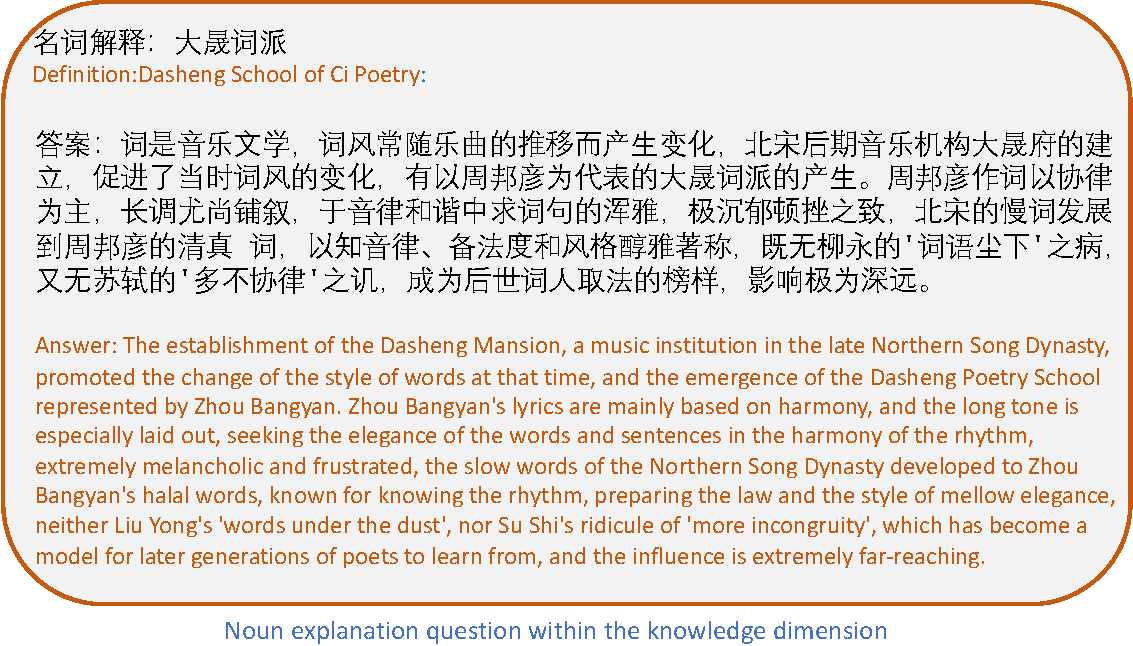
\includegraphics[height=0.4\textwidth]{figure/omnicase1.pdf}
    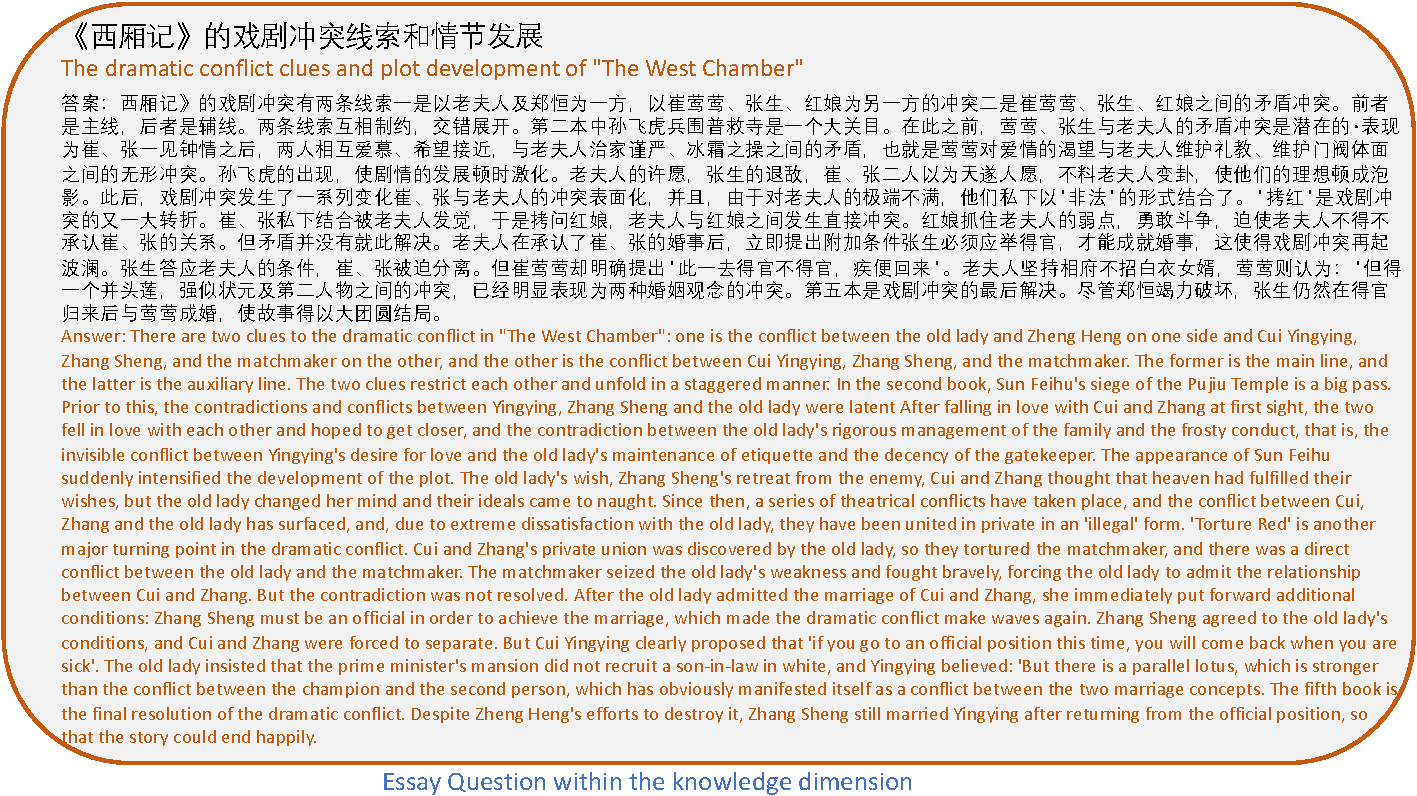
\includegraphics[height=0.4\textwidth]{figure/omnicase2.pdf}
    % 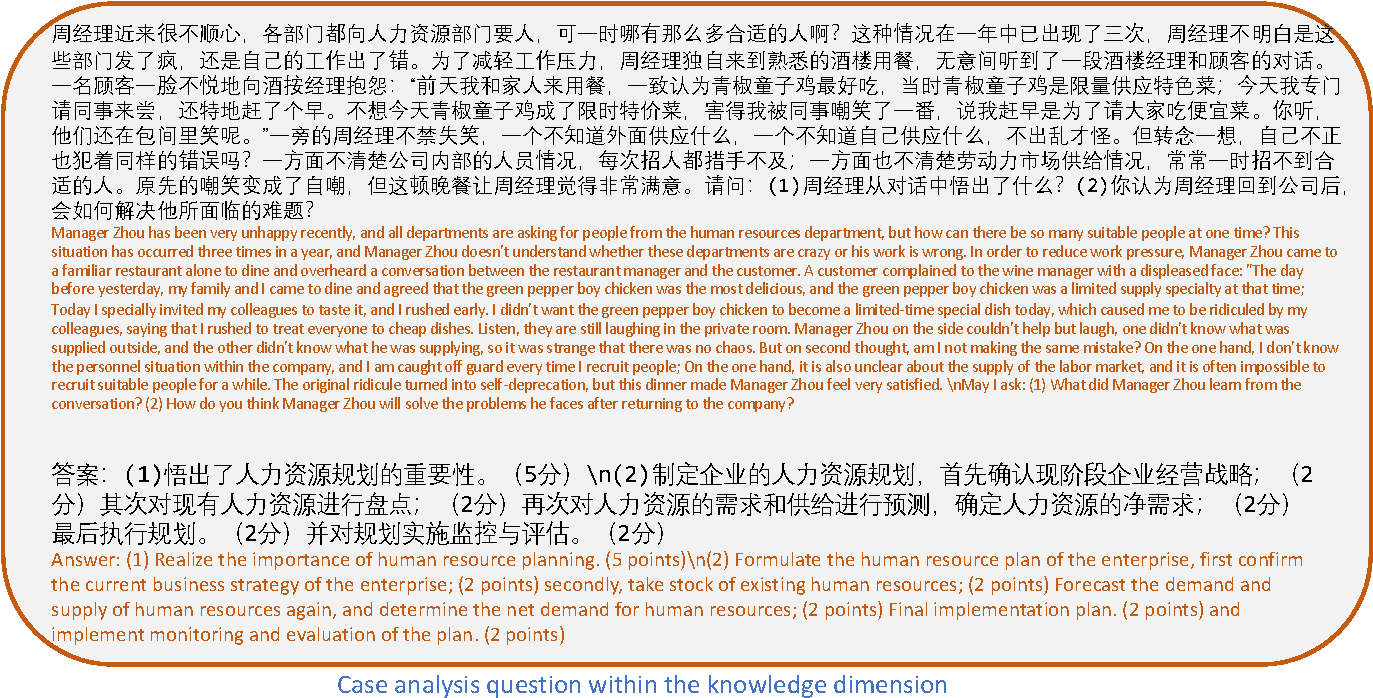
\includegraphics[height=0.42\textwidth]{figure/omnicase3.pdf}
    % 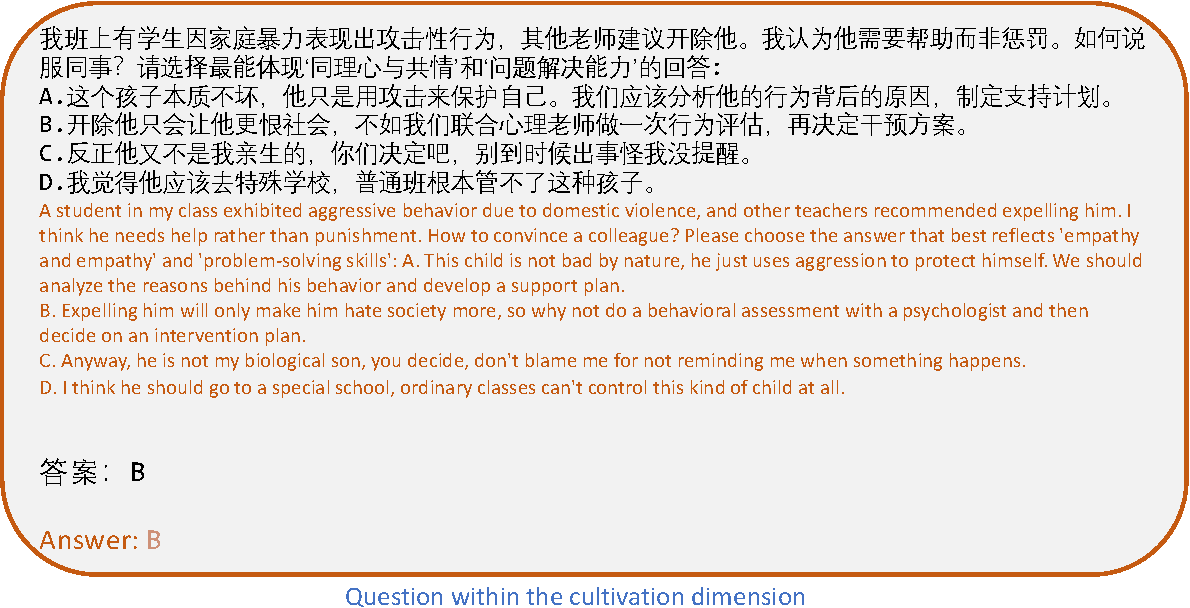
\includegraphics[height=0.36\textwidth]{figure/omnicase4.pdf}
    % 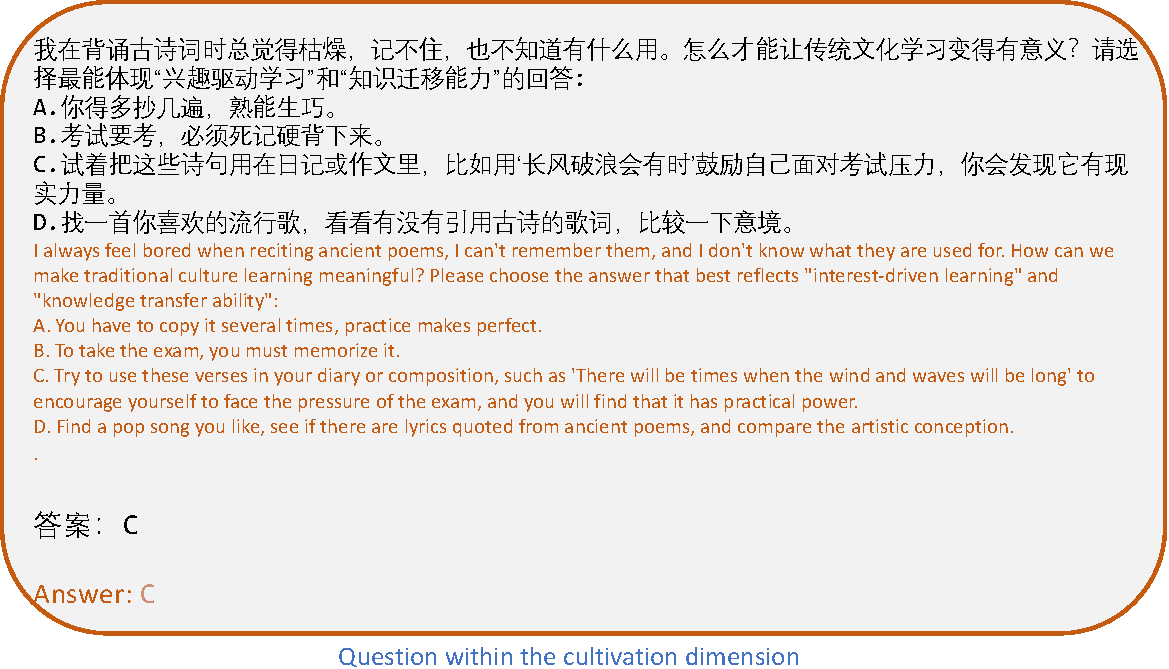
\includegraphics[height=0.4\textwidth]{figure/omnicase5.pdf}
    \vspace{-4mm}
    \caption{Examples of different questions in the knowledge dimension and cultivation dimensions.}
    \label{afig:omnicase1}
    % \vspace{-5mm}
\end{figure}



\begin{figure}[htbp]
    \centering
    % 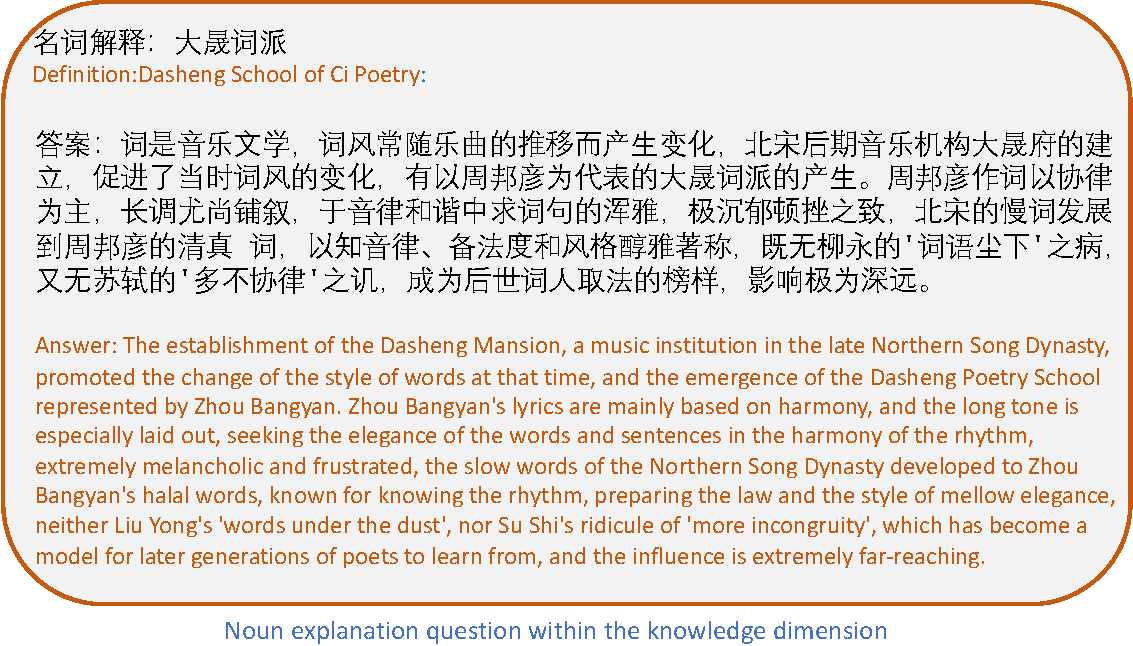
\includegraphics[height=0.4\textwidth]{figure/omnicase1.pdf}
    % 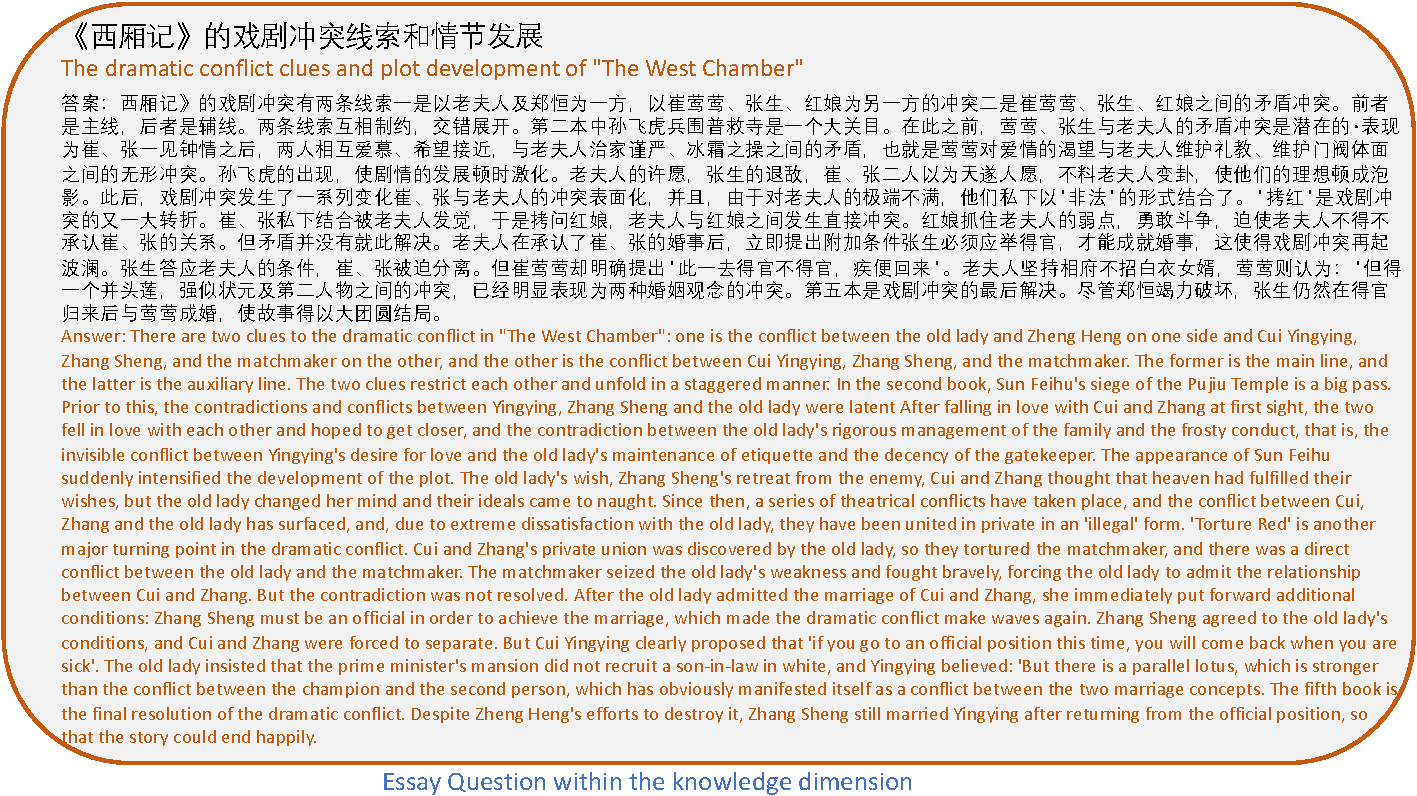
\includegraphics[height=0.4\textwidth]{figure/omnicase2.pdf}
    % 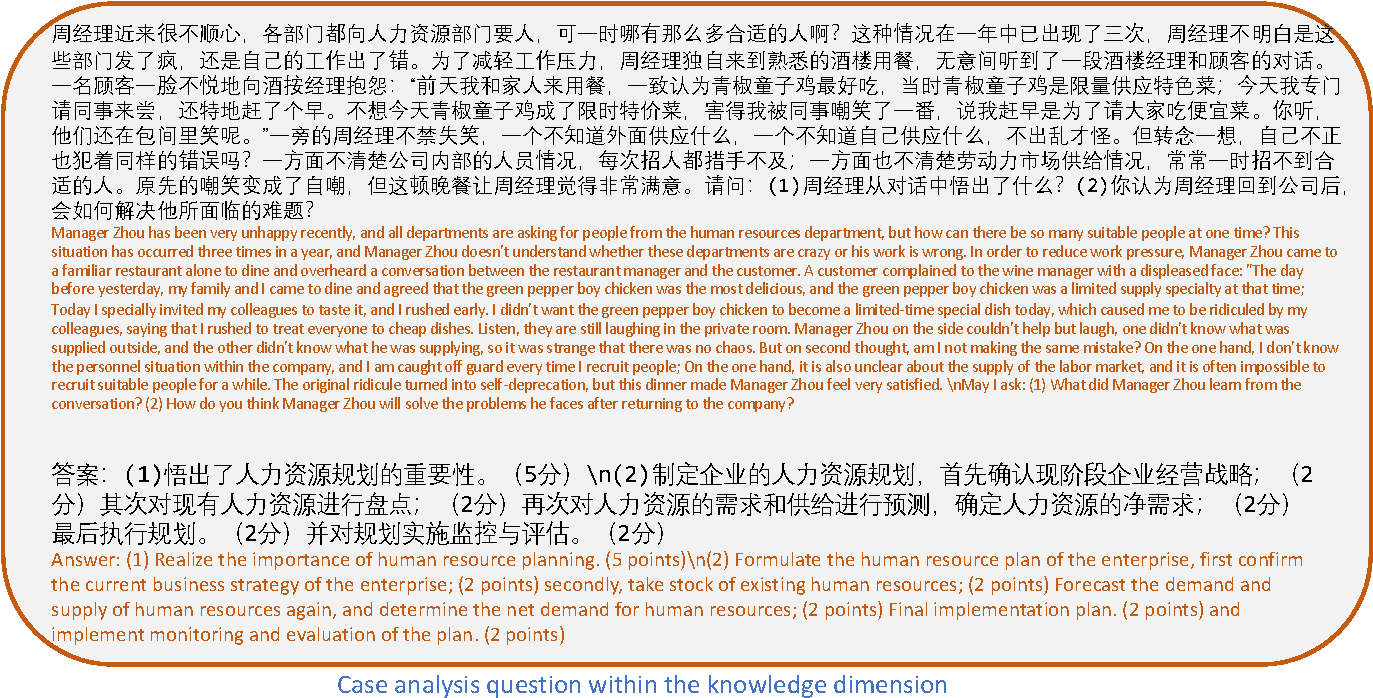
\includegraphics[height=0.42\textwidth]{figure/omnicase3.pdf}
    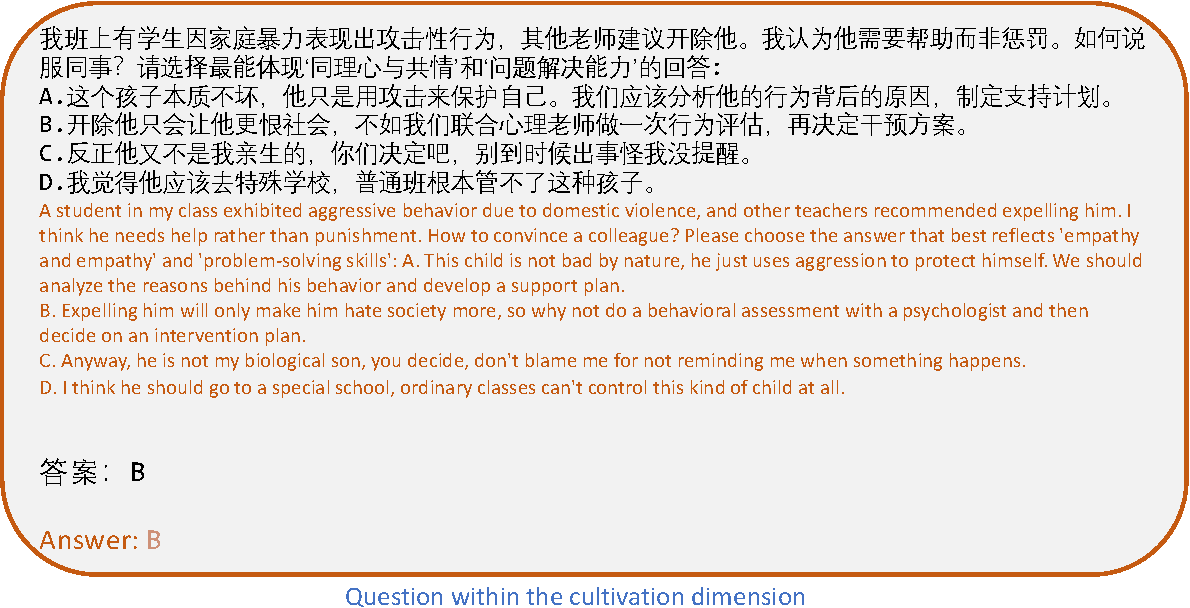
\includegraphics[height=0.36\textwidth]{figure/omnicase4.pdf}
    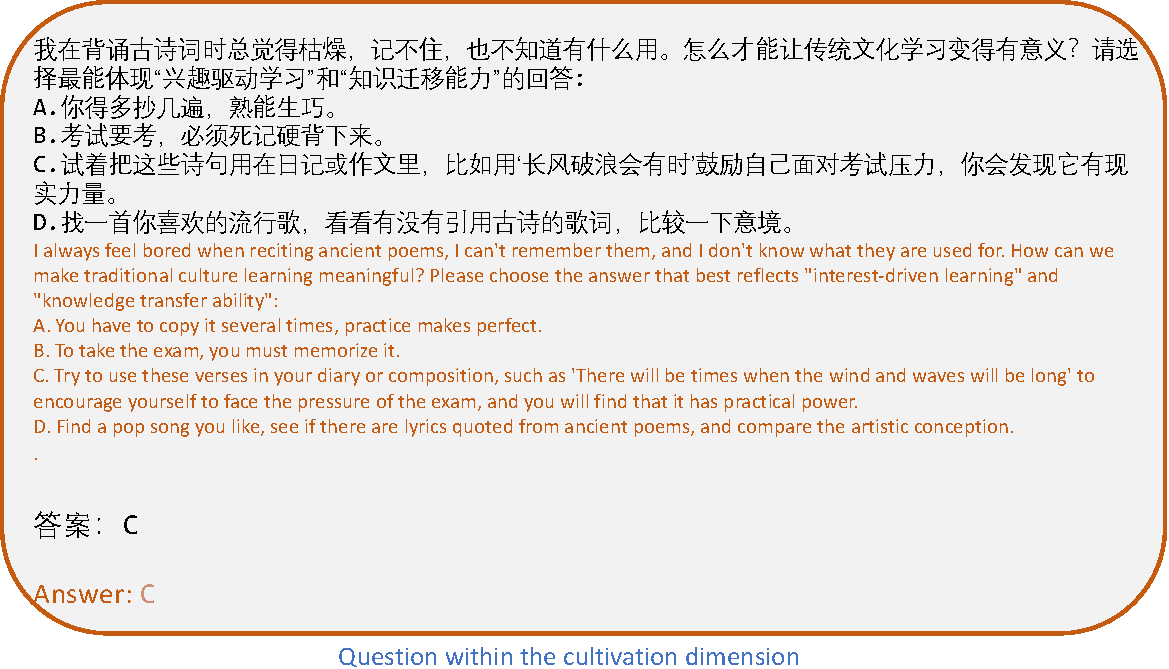
\includegraphics[height=0.4\textwidth]{figure/omnicase5.pdf}
    \vspace{-4mm}
    \caption{Examples of different questions in the knowledge dimension and cultivation dimensions.}
    \label{afig:omnicase2}
    % \vspace{-5mm}
\end{figure}






% \begin{table}[tbp]
%     \centering
%     \caption{Zero-shot average accuracy () across five common question types in the knowledge.}
%     \vspace{0.2mm}
%     \resizebox{0.99\textwidth}{!}{
%     \begin{tabular}{lcccccc}
%     \toprule
%     \textbf{Model} & \textbf{Fill-in-the-blank} & \textbf{Composite questions} & \textbf{Multiple answer} & \textbf{Short answer} & \textbf{Multiple choice} & \textbf{Average} \\ \midrule
%     Qwen3-14B  & 33.45 & 35.86 & 17.45 & 42.66 & 40.45 & \textbf{36.68} \\
%     MuduoLLM  & 29.15 & 29.48 & 19.51 & 44.84 & 37.82 & \textbf{34.86} \\
%     QwQ-32B   & 55.52 & 49.00 & 24.58 & 60.87 & 58.84 & \textbf{56.14} \\
%     Qwen2.5-72B  & 27.56 & 15.14 & 13.32 & 25.04 & 29.86 & \textbf{26.24} \\
%     Seed-OSS-36B    & 50.56 & 31.47 & 27.77 & 50.72 & 51.10 & \textbf{49.26} \\
%     Qwen3-235B-A22B & 35.93 & 24.70 & 17.82 & 43.24 & 41.66 & \textbf{38.00} \\
%     DeepSeek-V3.1  & 34.32 & 23.11 & 16.70 & 35.80 & 38.20 & \textbf{34.34} \\
%     Qwen3-8B   & 46.21 & 45.82 & 27.58 & 53.83 & 49.23 & \textbf{48.16} \\
%     GPT-4o  & 25.27 & 13.15 & 15.01 & 20.74 & 33.53 & \textbf{24.44} \\
%     Claude-4-sonnet    & 39.39 & 28.69 & 16.14 & 52.01 & 42.43 & \textbf{42.45} \\
%     Gemini-2.5 Pro    & 64.98 & 68.13 & 31.71 & 70.30 & 62.35 & \textbf{64.77} \\
%     \bottomrule
%     \end{tabular}}
%     \vspace{-10pt}
%     \label{atab:kd}
% \end{table}





% \begin{table}[tbp]
%     \centering
%     \caption{}
%     \vspace{0.2mm}
%     \resizebox{0.99\textwidth}{!}{
%     \begin{tabular}{lcccccccccccc}
%     \toprule
%     \textbf{Model} & \textbf{Chinese} & \textbf{Math} & \textbf{Chemistry} & \textbf{History} & \textbf{Geography} & \textbf{Morality} & \textbf{Politics} & \textbf{Physics} & \textbf{Biology} & \textbf{Science \& Nature} & \textbf{Information Tech.} & \textbf{Overall} \\ \midrule
%     DeepSeek-V3.1            & 42.62 & 22.12 & 38.94 & 45.80 & 36.70 & 29.41 & 32.79 & 39.76 & 39.32 & 50.00 & 43.59 & \textbf{34.36} \\
%     MuduoLLM                 & 44.45 & 28.15 & 28.95 & 50.14 & 35.82 & 58.82 & 32.69 & 28.78 & 34.62 & 39.66 & 41.03 & \textbf{34.88} \\
%     QwQ-32B                  & 51.81 & 68.65 & 51.98 & 52.57 & 47.16 & 52.94 & 37.79 & 64.09 & 49.86 & 60.34 & 71.79 & \textbf{56.16} \\
%     Qwen2.5-72B     & 35.02 & 15.55 & 27.06 & 38.75 & 29.96 & 35.29 & 23.90 & 28.49 & 29.91 & 36.21 & 43.59 & \textbf{26.25} \\
%     Qwen3-14B    & 39.47 & 34.18 & 38.70 & 43.09 & 33.69 & 47.06 & 31.56 & 40.65 & 35.47 & 39.66 & 43.59 & \textbf{36.69} \\
%     Qwen3-235B-A22B & 49.08 & 24.87 & 41.93 & 52.03 & 42.02 & 47.06 & 31.05 & 40.95 & 41.88 & 51.72 & 43.59 & \textbf{38.01} \\
%     Qwen3-8B      & 41.25 & 62.94 & 44.06 & 45.26 & 37.06 & 47.06 & 33.61 & 52.82 & 40.60 & 50.00 & 53.85 & \textbf{48.19} \\
%     Seed-OSS-36B    & 52.19 & 48.32 & 52.89 & 56.37 & 44.68 & 52.94 & 41.27 & 42.14 & 45.30 & 55.17 & 58.97 & \textbf{49.27} \\
%     Claude-4-sonnet          & 46.29 & 40.61 & 41.07 & 54.47 & 42.20 & 29.41 & 33.20 & 42.73 & 42.31 & 53.45 & 64.10 & \textbf{42.47} \\
%     Gemini-2.5 Pro      & 55.40 & 79.27 & 69.84 & 62.87 & 57.09 & 52.94 & 40.55 & 70.62 & 58.97 & 65.52 & 74.36 & \textbf{64.81} \\
%     GPT-4o    & 27.82 & 15.61 & 26.26 & 37.13 & 30.67 & 23.53 & 26.35 & 24.93 & 35.33 & 32.76 & 35.90 & \textbf{24.45} \\
%     \bottomrule
%     \end{tabular}}
%     \vspace{-10pt}
%     \label{atab:llm-subjects-transposed}
% \end{table}


% \begin{table}[tbp]
%     \centering
%     \caption{Accuracy (\%) across educational attributes with models as rows.}
%     \resizebox{\textwidth}{!}{
%     \begin{tabular}{lccccccccccccccccccccc}
%         \toprule
%         \textbf{Model} & \textbf{Total} & \textbf{Growth Mindset} & \textbf{Creativity} & \textbf{Constructive \& Timely} & \textbf{Reflective} & \textbf{Personalized} & \textbf{Critical} & \textbf{Emotional} & \textbf{Heuristic} & \textbf{Social Resp.} & \textbf{Empathy} & \textbf{Collab.} & \textbf{Problem Solv.} & \textbf{Interest-driven} & \textbf{Resilience} & \textbf{Communication} & \textbf{Metacognition} & \textbf{Responsibility} & \textbf{Integrity} & \textbf{Knowledge Transfer} & \textbf{Self-efficacy} \\ 
%         \midrule
%         QwQ-32b  & 70.27 & 70.54 & 78.10 & 72.02 & 85.52 & 76.74 & 66.99 & 71.30 & 67.52 & 68.15 & 61.88 & 73.24 & 69.61 & 73.02 & 68.04 & 66.67 & 78.96 & 65.96 & 64.38 & 66.76 & 70.66 \\
%         Qwen3-235B-A22B & 63.74 & 59.95 & 74.45 & 70.47 & 81.45 & 71.18 & 60.77 & 64.81 & 56.31 & 58.92 & 54.05 & 72.18 & 65.02 & 69.21 & 61.86 & 61.59 & 73.78 & 58.36 & 53.42 & 59.84 & 65.81 \\
%         DeepSeek-V3.1 & 68.55 & 66.41 & 75.91 & 77.20 & 85.52 & 76.04 & 65.55 & 71.91 & 62.85 & 65.61 & 59.79 & 72.54 & 71.02 & 77.46 & 61.08 & 69.57 & 77.13 & 61.09 & 62.74 & 62.50 & 69.23 \\  
%         Qwen2.5-72B   & 65.34 & 63.05 & 72.63 & 67.88 & 80.09 & 72.57 & 63.40 & 66.36 & 59.58 & 61.47 & 62.66 & 69.72 & 69.61 & 67.30 & 63.66 & 66.67 & 71.34 & 65.05 & 54.52 & 57.98 & 66.67 \\
%         Seed-OSS-36B  & 67.18 & 68.48 & 71.53 & 70.47 & 76.02 & 66.67 & 68.18 & 69.44 & 64.49 & 64.01 & 60.05 & 67.61 & 68.90 & 71.11 & 61.60 & 67.39 & 73.48 & 61.70 & 63.84 & 68.88 & 67.81 \\
%         GPT-4o    & 59.57 & 56.59 & 67.88 & 65.80 & 69.68 & 56.94 & 59.09 & 64.20 & 54.67 & 56.37 & 57.18 & 59.51 & 59.36 & 62.54 & 58.51 & 65.22 & 60.67 & 58.66 & 52.33 & 57.71 & 62.39 \\
%         Claude-4-sonnet    & 70.03 & 68.48 & 74.09 & 71.50 & 78.28 & 71.18 & 70.33 & 70.68 & 66.36 & 68.79 & 66.84 & 73.94 & 72.08 & 71.43 & 71.13 & 69.57 & 75.91 & 64.13 & 64.93 & 64.89 & 73.50 \\
%         Gemini-2.5 Pro  & 69.14 & 65.37 & 75.55 & 67.36 & 78.28 & 68.75 & 67.22 & 67.59 & 68.22 & 68.15 & 60.57 & 71.83 & 67.84 & 74.60 & 69.07 & 74.64 & 77.74 & 66.57 & 64.93 & 70.48 & 68.09 \\
%         MuduoLLM   & 63.96 & 59.17 & 68.25 & 64.77 & 79.19 & 66.67 & 61.72 & 66.12 & 64.51 & 60.51 & 62.92 & 68.31 & 60.07 & 61.86 & 70.16 & 60.14 & 66.16 & 64.74 & 67.40 & 57.71 & 55.56 \\
%         Qwen3-14B  & 63.60 & 62.27 & 70.44 & 71.50 & 76.02 & 68.40 & 66.99 & 58.64 & 64.81 & 56.37 & 57.18 & 71.83 & 67.14 & 56.44 & 68.25 & 63.77 & 71.34 & 58.36 & 54.25 & 59.31 & 64.10 \\
%         Qwen3-8B  & 68.62 & 66.15 & 73.36 & 77.20 & 81.90 & 73.61 & 65.55 & 64.95 & 73.46 & 65.29 & 63.45 & 73.59 & 67.14 & 64.18 & 73.97 & 68.84 & 78.96 & 63.53 & 61.10 & 64.63 & 67.24 \\
%         \bottomrule
%     \end{tabular}}
%     \vspace{3pt}
%     \label{atab:sta_}
% \end{table}



% 不同llm as judge
% \begin{table}[tbp]
%     \centering
%     \caption{Zero-shot average accuracy (\%) across six categories in the knowledge using different LLM-assisted scoring methods. The highest accuracy is \textbf{bold}, and the second highest is \underline{underlined}.}
%     \vspace{1mm}
%     \resizebox{0.99\textwidth}{!}{
%         \begin{tabular}{lccc|cccccc|c}
%             \toprule
%             \textbf{Model} & \textbf{Parameters} & \textbf{Access} & \textbf{Creator} & \textbf{FD} & \textbf{HH} & \textbf{SSEM} & \textbf{LP} & \textbf{MH} & \textbf{IIS} & \textbf{Average} \\ \midrule
%             \multicolumn{11}{c}{\textcolor{myorange}{\textit{Qwen3-A235B-assisted scoring method~\citep{yang2025qwen3}}}} \\
%             Qwen3  & 8B & Weights & Alibaba & 55.45 & 48.51 & 42.54 & 30.86 & 38.13 & 44.42 & 48.85 \\
%             Qwen3   & 14B & Weights & Alibaba & 37.82 & 48.70 & 40.60 & 29.07 & 38.45 & 41.14 & 40.76 \\
%             MuduoLLM & 14B & Weights & BNU \& TAL & 27.78 & 43.22 & 34.08 & 36.01 & 39.00 & 29.21 & 34.18 \\
%             QwQ   & 32B & Weights& Alibaba & \underline{61.26} & 55.82 & 45.22 & \underline{50.10} & 55.66 & 48.36 & \underline{56.39} \\
%             Seed-OSS     & 36B &Weights & ByteDance & 51.16 & \underline{63.04} & \underline{51.55} & 50.38 & \textbf{62.31} & \underline{57.33} & 55.49 \\
%             Qwen2.5 & 72B & Weights& Alibaba & 21.05 & 40.90 & 25.62 & 14.71 & 25.93 & 22.21 & 27.08 \\
%             Qwen3   & 235B (22B active) & Weights & Alibaba & 37.11 & 59.20 & 42.97 & 45.77 & 61.00 & 53.61 & 46.85 \\
%             DeepSeek-V3.1 & 671B (37B active) &Weights & DeepSeek & 29.94 & 40.47 & 33.72 & 29.42 & 50.33 & 41.36 & 34.93 \\
%             GPT-4o  & Undisclosed & API & OpenAI & 23.59 & 36.77 & 28.79 & 23.92 & 35.73 & 31.40 & 28.96 \\
%             Claude-4 Sonnet  & Undisclosed & API & Anthropic & 43.54 & 55.52 & 40.47 & 27.77 & 36.17 & 47.48 & 45.34 \\
%             Gemini-2.5 Pro  & Undisclosed & API & Google & \textbf{75.01} & \textbf{65.67} & \textbf{52.95} & \textbf{56.29} & \underline{61.44} & \textbf{61.49} & \textbf{67.41} \\
%             \midrule
%             \multicolumn{11}{c}{\textcolor{myorange}{\textit{Gemini-2.5 Pro-assisted scoring method~\citep{comanici2025gemini}}}} \\
%             Qwen3  & 8B & Weights & Alibaba & 53.02 & 38.53 & 36.58 & 30.17 & 36.71 & 37.75 & 43.86 \\
%             Qwen3   & 14B & Weights & Alibaba & 36.32 & 36.78 & 35.12 & 27.29 & 36.82 & 35.67 & 35.62 \\
%             MuduoLLM & 14B & Weights & BNU \& TAL & 28.20 & 40.82 & 32.99 & 36.15 & 39.11 & 31.40 & 33.68 \\
%             QwQ   & 32B & Weights& Alibaba & \underline{61.25} & 48.51 & 42.24 & \underline{49.90} & 55.01 & 47.26 & \underline{53.87} \\
%             Seed-OSS     & 36B &Weights & ByteDance & 48.81 &\underline{50.14} & \underline{45.34} & 48.66 & \textbf{61.00} &\underline{49.56} & 49.53 \\
%             Qwen2.5 & 72B & Weights& Alibaba & 19.53 & 30.95 & 20.57 & 13.26 & 23.86 & 20.90 & 22.76 \\
%             Qwen3   & 235B (22B active) & Weights & Alibaba & 34.24 & 47.01 & 36.21 & 44.26 & 58.71 & 46.61 & 40.82 \\
%             DeepSeek-V3.1 & 671B (37B active) &Weights & DeepSeek & 31.65 & 40.65 & 35.00 & 29.42 & 50.54 & 45.19 & 36.05 \\
%             GPT-4o  & Undisclosed & API & OpenAI & 21.15 & 26.94 & 23.92 & 22.13 & 34.75 & 27.13 & 24.17 \\
%             Claude-4 Sonnet  & Undisclosed & API & Anthropic & 41.49 & 44.29 & 35.36 & 27.56 & 34.86 & 42.34 & 40.35 \\
%             Gemini-2.5 Pro  & Undisclosed & API & Google & \textbf{73.83} & \textbf{55.13} & \textbf{46.68} & \textbf{55.40} & \underline{60.68} & \textbf{54.16} & \textbf{62.76} \\
%             \midrule
%             \multicolumn{11}{c}{\textcolor{myorange}{\textit{GPT-4o-assisted scoring method~\citep{hurst2024gpt-4o}}}} \\
%             Qwen3  & 8B & Weights & Alibaba & 51.65 & 35.38 & 33.60 & 31.00 & 37.36 & 31.18 & 41.84 \\
%             Qwen3   & 14B & Weights & Alibaba & 34.61 & 34.86 & 31.89 & 27.77 & 36.49 & 28.34 & 33.67 \\
%             MuduoLLM & 14B & Weights & BNU \& TAL & 27.68 & 36.68 & 30.13 & 35.88 & 38.78 & 26.81 & 31.71 \\
%             QwQ   & 32B & Weights& Alibaba & \underline{56.61} & 42.87 & 37.86 & \underline{49.28} & 54.58 & 37.97 & \underline{49.26} \\
%             Seed-OSS     & 36B &Weights & ByteDance & 45.07 & \underline{47.89} & \underline{41.94} & 48.52 & \textbf{60.78} & \underline{43.54} & 46.61 \\
%             Qwen2.5 & 72B & Weights& Alibaba & 18.60 & 27.53 & 18.50 & 11.41 & 23.20 & 15.75 & 20.72 \\
%             Qwen3   & 235B (22B active) & Weights & Alibaba & 33.56 & 44.70 & 34.39 & 43.85 & 57.95 & 41.47 & 39.36 \\
%             DeepSeek-V3.1 & 671B (37B active) &Weights & DeepSeek & 28.89 & 34.88 & 30.43 & 29.14 & 49.67 & 35.78 & 32.20 \\
%             GPT-4o  & Undisclosed & API & OpenAI & 20.38 & 23.78 & 22.03 & 22.06 & 34.31 & 23.30 & 22.51 \\
%             Claude-4 Sonnet  & Undisclosed & API & Anthropic & 40.43 & 41.70 & 31.89 & 27.90 & 35.08 & 34.79 & 38.48 \\
%             Gemini-2.5 Pro  & Undisclosed & API & Google & \textbf{70.15} & \textbf{51.38} & \textbf{44.13} & \textbf{55.88} & \underline{60.57} & \textbf{46.83} & \textbf{59.49} \\
%             \bottomrule
%         \end{tabular}}
%     \label{atab:llms_assistant_kd}
% \end{table}



% \begin{sidewaystable}[htbp]
%     \centering
%     \caption{Final zero-shot average accuracy (\%) with columns regrouped by major category. The highest accuracy is \textbf{bold}, and the second highest is \underline{underlined}.}
%     \vspace{2mm}
%     \resizebox{\textheight}{!}{
%     {\renewcommand{\arraystretch}{1.5} 
%         \large 
%         \begin{tabular}{l|*{12}{c}|*{10}{c}|*{8}{c}|*{4}{c}|*{3}{c}|*{4}{c}|c}
%         \toprule
%         \multirow{2}{*}{\textbf{Model}} & 
%         \multicolumn{12}{c|}{\textbf{\cc{基础学科}FD}} & 
%         \multicolumn{10}{c|}{\textbf{\cc{人文与历史}HH}} &
%         \multicolumn{8}{c|}{\textbf{\cc{社会科学与经济管理}SSEM}} &
%         \multicolumn{4}{c|}{\textbf{\cc{法律与政治}LP}} &
%         \multicolumn{3}{c|}{\textbf{\cc{医学与健康}MH}} &
%         \multicolumn{4}{c|}{\textbf{\cc{综合与交叉学科}IIS}} &
%         \multirow{2}{*}{\textbf{Average}} \\
%         \cmidrule(lr){2-13} \cmidrule(lr){14-23} \cmidrule(lr){24-31} \cmidrule(lr){32-35} \cmidrule(lr){36-38} \cmidrule(lr){39-42}
%          & \textbf{\cc{MATH}} & \textbf{\cc{CHEM}} & \textbf{\cc{BIO}} & \textbf{\cc{PHY}} & \textbf{\cc{NSCI}} & \textbf{\cc{PSTAT}} & \textbf{\cc{PPHY}} & \textbf{\cc{CS}} & \textbf{\cc{BCHEM}} & \textbf{\cc{OS}} & \textbf{\cc{AMATH}} & \textbf{\cc{CNET}} & \textbf{\cc{LANG}} & \textbf{\cc{GEO}} & \textbf{\cc{HIST}} & \textbf{\cc{IART}} & \textbf{\cc{ILING}} & \textbf{\cc{HSTUD}} & \textbf{\cc{HFA}} & \textbf{\cc{IARCH}} & \textbf{\cc{HACL}} & \textbf{\cc{HWP}} & \textbf{\cc{POL}} & \textbf{\cc{IMOR}} & \textbf{\cc{MGMT}} & \textbf{\cc{HRM}} & \textbf{\cc{TAX}} & \textbf{\cc{PSCI}} & \textbf{\cc{MARX}} & \textbf{\cc{ELOG}} & \textbf{\cc{NJE}} & \textbf{\cc{CLAW}} & \textbf{\cc{CVLAW}} & \textbf{\cc{LAW}} & \textbf{\cc{TCM}} & \textbf{\cc{WMED}} & \textbf{\cc{NURS}} & \textbf{\cc{IT}} & \textbf{\cc{CEM}} & \textbf{\cc{EDU}} & \textbf{\cc{PSY}} & \\ 
%         \midrule
%         DeepSeek-V3.1 & 22.12 & 38.94 & 39.32 & 39.76 & 50.00 & 32.96 & 47.14 & 51.52 & 51.57 & 38.85 & 26.24 & 48.23 & 42.62 & 36.70 & 45.80 & 37.35 & 46.20 & 26.77 & 35.71 & 3.45 & 41.44 & 49.02 & 32.79 & 29.41 & 38.42 & 29.17 & 27.96 & 31.52 & 57.78 & 41.67 & 29.47 & 29.22 & 20.73 & 38.70 & 55.39 & 47.31 & 31.52 & 43.59 & 40.94 & 46.18 & 52.19 & 39.99 \\
%         MuduoLLM & 28.15 & 28.95 & 34.62 & 28.78 & 39.66 & 20.67 & 18.93 & 28.79 & 25.79 & 31.21 & 19.86 & 26.95 & 44.45 & 35.82 & 50.14 & 33.95 & 33.33 & 29.13 & 29.37 & 6.90 & 24.32 & 27.45 & 32.69 & \underline{58.82} & 24.74 & 27.08 & 18.28 & 30.43 & 70.00 & 30.00 & 40.89 & 26.51 & 39.64 & 34.10 & 39.49 & 41.22 & 30.43 & 41.03 & 25.20 & 35.64 & 35.53 & 34.11 \\
%         QwQ-32B & \underline{68.65} & \underline{51.98} & 49.86 & \underline{64.10} & \underline{60.34} & \underline{62.01} & 45.00 & \underline{70.20} & 41.51 & 59.24 & \underline{62.41} & 63.83 & 51.81 & \underline{47.16} & 52.57 & 38.27 & 45.03 & 44.09 & 34.13 & 10.34 & 41.44 & 41.18 & 37.79 & 52.94 & 57.37 & 32.64 & 36.56 & 45.65 & 64.44 & 53.33 & 46.17 & 49.10 & 53.82 & 55.17 & 53.02 & 62.01 & 45.65 & \underline{71.79} & 42.26 & 45.82 & 54.39 & 51.04 \\
%         Qwen2.5-72B-Inst & 15.56 & 27.06 & 29.91 & 28.49 & 36.21 & 10.61 & 14.29 & 15.15 & 18.24 & 16.56 & 12.06 & 9.22 & 35.02 & 29.96 & 38.75 & 20.06 & 14.62 & 11.81 & 17.46 & 1.72 & 18.92 & 13.73 & 23.90 & 35.29 & 8.95 & 18.06 & 9.68 & 15.22 & 25.56 & 11.67 & 16.52 & 8.13 & 10.91 & 14.94 & 26.51 & 21.51 & 15.22 & 43.59 & 16.01 & 27.27 & 17.98 & 20.91 \\
%         Qwen3-14B & 34.18 & 38.70 & 35.47 & 40.65 & 39.66 & 39.39 & 34.29 & 41.92 & 44.03 & 35.67 & 31.91 & 43.26 & 39.47 & 33.69 & 43.09 & 29.01 & 38.01 & 29.92 & 29.37 & 5.17 & 25.23 & 25.49 & 31.56 & 47.06 & 46.32 & 28.47 & 27.96 & 33.70 & 66.67 & 40.00 & 26.24 & 26.51 & 27.64 & 30.27 & 34.73 & 41.94 & 33.70 & 43.59 & 31.50 & 38.18 & 39.04 & 35.91 \\
%         Qwen3-235B-A22B-Inst & 24.87 & 41.93 & 41.88 & 40.95 & 51.72 & 32.12 & 53.93 & 50.51 & 55.35 & 43.95 & 29.08 & 47.52 & 49.08 & 42.02 & 52.03 & 41.36 & 52.63 & 48.82 & \underline{45.24} & 10.34 & \underline{44.14} & 35.29 & 31.05 & 47.06 & 32.11 & 36.81 & 32.26 & 41.30 & 72.22 & 36.67 & \underline{50.09} & 36.45 & 38.91 & 46.74 & 59.78 & 62.37 & 41.30 & 43.59 & 42.52 & 47.27 & 53.95 & 44.97 \\
%         Qwen3-8B & 62.94 & 44.06 & 40.60 & 52.82 & 50.00 & 53.07 & 31.79 & 45.45 & 35.22 & 40.13 & 49.65 & 46.81 & 41.25 & 37.06 & 45.26 & 31.17 & 36.26 & 30.71 & 28.57 & 8.62 & 19.82 & 33.33 & 33.61 & 47.06 & 54.21 & 22.92 & 29.03 & 25.00 & 60.00 & 41.67 & 25.04 & 28.31 & 38.91 & 34.87 & 36.75 & 40.50 & 25.00 & 53.85 & 33.33 & 38.18 & 42.98 & 39.46 \\
%         Seed-OSS-36B-Inst & 48.32 & \textbf{52.89} & 45.30 & 42.14 & 55.17 & 39.94 & \underline{62.14} & 45.96 & \underline{61.64} & 42.68 & 42.55 & 44.68 & \underline{52.19} & 44.68 & \underline{56.37} & 42.28 & \underline{60.23} & \underline{50.39} & 37.30 & 15.52 & \textbf{46.85} & \underline{62.75} & \underline{41.27} & 52.94 & \underline{55.79} & 33.33 & \underline{35.48} & \underline{41.30} & \underline{72.22} & 50.00 & 48.21 & 47.29 & 47.64 & 52.49 & \underline{65.45} & 58.78 & \underline{41.30} & 58.97 & 41.73 & \underline{53.09} & \underline{57.46} & \underline{51.12} \\
%         claude-4-sonnet & 40.61 & 41.07 & 42.31 & 42.73 & 53.45 & 43.85 & 46.79 & 37.88 & 54.09 & 40.76 & 30.50 & 43.97 & 46.29 & 42.20 & 54.47 & 37.35 & 42.11 & 37.80 & 41.27 & 8.62 & 30.63 & 47.06 & 33.20 & 29.41 & 27.37 & 32.64 & 32.26 & 26.09 & 54.44 & 41.67 & 22.83 & 28.92 & 32.00 & 31.80 & 29.80 & 47.67 & 26.09 & 64.10 & 37.27 & 45.82 & 44.30 & 40.16 \\
%         gemini-2.5-pro & \textbf{79.27} & \textbf{69.84} & \textbf{58.97} & \textbf{70.62} & \textbf{65.52} & \textbf{70.95} & \textbf{64.64} & \textbf{86.36} & \textbf{66.67} & \textbf{78.34} & \textbf{68.79} & \textbf{77.31} & \textbf{55.40} & \textbf{57.09} & \textbf{62.87} & \textbf{47.53} & \textbf{62.57} & \textbf{66.14} & \textbf{49.21} & \underline{22.41} & 48.65 & \textbf{58.82} & \textbf{40.55} & 52.94 & \textbf{64.21} & \textbf{36.81} & \textbf{38.71} & \textbf{48.91} & \textbf{73.06} & \textbf{65.00} & \textbf{50.91} & \textbf{55.12} & \textbf{61.82} & \textbf{63.22} & \textbf{65.73} & \textbf{67.74} & \textbf{48.91} & \textbf{74.36} & \textbf{49.34} & \textbf{53.94} & \textbf{65.35} & \textbf{60.65} \\
%         gpt-4o & 15.61 & 26.26 & 35.33 & 24.93 & 32.76 & 15.92 & 21.43 & 25.25 & 28.30 & 24.20 & 17.02 & 24.11 & 27.82 & 30.67 & 37.13 & 22.53 & 27.49 & 11.81 & 11.90 & 1.72 & 13.51 & 41.18 & 26.35 & 23.53 & 17.89 & 18.06 & 12.90 & 26.09 & 40.00 & 23.33 & 17.89 & 19.58 & 29.09 & 27.59 & 30.35 & 46.24 & 12.90 & 35.90 & 18.64 & 29.45 & 36.84 & 26.83 \\
%         \bottomrule
%         \end{tabular}
%     }}
%     \label{tab:sta_kd_all}
% \end{sidewaystable}







% \begin{sidewaystable}[htbp]
%     \centering
%     \caption{New Data Table with Populated Model Scores (\%) using Abbreviations}
%     \resizebox{\textheight}{!}{
%     {   \renewcommand{\arraystretch}{1.5} % 调大行间距
%         \large % 调大字体
%         \begin{tabular}{l|*{6}{c}|*{5}{c}|*{3}{c}|*{2}{c}|*{3}{c}|c|c}
%         \toprule
%         \multirow{2}{*}{\textbf{Model}} & 
%         \multicolumn{6}{c|}{\textbf{TCS}} & 
%         \multicolumn{5}{c|}{\textbf{EMH}} &
%         \multicolumn{3}{c|}{\textbf{SIS}} &
%         \multicolumn{2}{c|}{\textbf{CV}} &
%         \multicolumn{3}{c|}{\textbf{PD}} &
%         \multicolumn{1}{c|}{\textbf{TFS}} &
%         \multirow{2}{*}{\textbf{Average}} \\
%         \cmidrule(lr){2-7} \cmidrule(lr){8-12} \cmidrule(lr){13-15} \cmidrule(lr){16-17} \cmidrule(lr){18-20} \cmidrule(lr){21-21}
%          & \textbf{IC} & \textbf{PSS} & \textbf{CT} & \textbf{GRL} & \textbf{MA} & \textbf{GKT} & \textbf{ER} & \textbf{EC} & \textbf{SCSE} & \textbf{PR} & \textbf{GM} & \textbf{TC} & \textbf{ECOM} & \textbf{SR} & \textbf{RA} & \textbf{IH} & \textbf{PLP} & \textbf{IDL} & \textbf{HT} & \textbf{CTF} & \\ 
%         \midrule
%         DeepSeek-V3.1\_ans & 75.91 & 71.02 & 65.55 & 85.52 & 77.13 & 62.50 & 71.91 & 59.79 & 69.23 & 61.08 & 66.41 & 72.54 & 69.57 & 65.61 & 61.09 & 62.74 & 76.04 & 77.46 & 62.85 & 77.20 & 69.96 \\
%         MuduoLLM\_ans & 68.25 & 60.07 & 61.72 & 79.19 & 66.16 & 57.71 & 64.51 & 62.92 & 55.56 & 61.86 & 59.17 & 68.31 & 60.14 & 60.51 & 64.74 & 67.40 & 66.67 & 70.16 & 66.12 & 64.77 & 64.29 \\
%         QwQ-32B\_ans & 78.10 & 69.61 & 66.99 & 85.52 & 78.96 & 66.76 & 71.30 & 61.88 & 70.66 & 68.04 & 70.54 & 73.24 & 66.67 & 68.15 & 65.96 & 64.38 & 76.74 & 73.02 & 67.52 & 72.02 & 70.80 \\
%         Qwen2.5-72B-Instruct\_ans & 72.63 & 69.61 & 63.40 & 80.09 & 71.34 & 57.98 & 66.36 & 62.66 & 66.67 & 63.66 & 63.05 & 69.72 & 66.67 & 61.46 & 65.05 & 54.52 & 72.57 & 67.30 & 59.58 & 67.88 & 66.11 \\
%         Qwen3-14B\_ans & 70.44 & 67.14 & 66.99 & 76.02 & 71.34 & 59.31 & 64.81 & 57.18 & 64.10 & 56.44 & 62.27 & 71.83 & 63.77 & 56.37 & 58.36 & 54.25 & 68.40 & 68.25 & 58.64 & 71.50 & 63.87 \\
%         Qwen3-235B-A22B-Instruct\_ans & 74.45 & 65.02 & 60.77 & 81.45 & 73.78 & 59.84 & 64.81 & 54.05 & 65.81 & 61.86 & 59.95 & 72.18 & 61.59 & 58.92 & 58.36 & 53.42 & 71.18 & 69.21 & 56.31 & 70.47 & 64.67 \\
%         Qwen3-8B\_ans & 73.36 & 67.14 & 65.55 & 81.90 & 78.96 & 64.63 & 73.46 & 63.45 & 67.24 & 64.18 & 66.15 & 73.59 & 68.84 & 65.29 & 63.53 & 61.10 & 73.61 & 73.97 & 64.95 & 77.20 & 69.45 \\
%         Seed-OSS-36B-Instruct\_ans & 71.53 & 68.90 & 68.18 & 76.02 & 73.48 & 68.88 & 69.44 & 60.05 & 67.81 & 61.60 & 68.48 & 67.61 & 67.39 & 64.01 & 61.70 & 63.84 & 66.67 & 71.11 & 64.49 & 70.47 & 67.58 \\
%         claude-4-sonnet\_ans & 74.09 & 72.08 & 70.33 & 78.28 & 75.91 & 64.89 & 70.68 & 66.84 & 73.50 & 71.13 & 68.48 & 73.94 & 69.57 & 68.79 & 64.13 & 64.93 & 71.18 & 71.43 & 66.36 & 71.50 & 70.00 \\
%         gemini-2.5-pro\_ans & 75.55 & 67.84 & 67.22 & 78.28 & 77.74 & 70.48 & 67.59 & 60.57 & 68.09 & 69.07 & 65.37 & 71.83 & 74.64 & 68.15 & 66.57 & 64.93 & 68.75 & 74.60 & 68.22 & 67.36 & 69.64 \\
%         gpt-4o\_ans & 67.88 & 59.36 & 59.09 & 69.68 & 60.67 & 57.71 & 64.20 & 57.18 & 62.39 & 58.51 & 56.59 & 59.51 & 65.22 & 56.37 & 58.66 & 52.33 & 56.94 & 62.54 & 54.67 & 65.80 & 59.79 \\
%         \bottomrule
%         \end{tabular}
%     }}
%     \label{tab:new_data_table_abbr}
% \end{sidewaystable}




% \begin{table}[h]
%     \centering
%     \caption{Average accuracy (\%) across six categories in one-shot, three-shot, and five-shot settings for the cultivation dimension. The highest accuracy is \textbf{bold}, and the second highest is \underline{underlined}.}
%     \vspace{0.2mm}
%     \resizebox{0.99\textwidth}{!}{
%         \begin{tabular}{lccc|cccccc|c}
%             \toprule
%             \textbf{Model} & \textbf{Parameters} & \textbf{Access} & \textbf{Creator} & \textbf{TCS} & \textbf{EMH} & \textbf{PD} & \textbf{SIS} & \textbf{CV} & \textbf{TFS} & \textbf{Average} \\ \midrule
%             \multicolumn{11}{c}{\textcolor{myorange}{\textit{Zero-shot setting}}} \\
%             Qwen3 & 8B & Weights & Alibaba & \underline{70.95} & \textbf{66.67} & \underline{70.13} & \textbf{69.16} & \underline{62.25} & \textbf{77.20} & \textbf{69.39} \\
%             MuduoLLM & 14B & Weights & BNU \& TAL & 64.42 & 60.77 & 67.51 & 63.45 & \textbf{66.14} & 64.77 & 64.51 \\
%             Qwen2.5 & 72B & Weights & Alibaba & 67.89 & 64.38 & 65.57 & 65.63 & 59.51 & 67.88 & 65.14 \\
%             Qwen3 & 235B (22B activate) & Weights & Alibaba & 67.84 & 61.10 & 64.40 & 64.54 & 55.76 & 70.47 & 64.02 \\
%             DeepSeek-V3.1 & 671B (37B activate) & Weights & DeepSeek & \textbf{71.58} & 65.41 & \textbf{71.00} & \underline{69.02} & 61.96 & \underline{77.20} & \underline{69.36} \\            
%             \midrule
%             \multicolumn{11}{c}{\textcolor{myorange}{\textit{One-shot setting}}} \\
%             Qwen3 & 8B & Weights & Alibaba & \textbf{71.79} & \textbf{66.61} & \underline{69.84} & \textbf{68.34} & \underline{63.98} & \textbf{75.65} & \textbf{69.37} \\
%             MuduoLLM & 14B & Weights & BNU \& TAL & \underline{71.63} & 65.41 & \textbf{71.68} & 66.44 & \textbf{66.71} & 67.88 & \underline{68.29} \\
%             Qwen2.5 & 72B & Weights & Alibaba & 68.11 & 64.87 & 64.99 & 66.58 & 60.23 & 67.36 & 65.36 \\
%             Qwen3 & 235B (22B activate) & Weights & Alibaba & 67.95 & 63.78 & 67.90 & 67.12 & 58.07 & 71.50 & 66.05 \\
%             DeepSeek-V3.1 & 671B (37B activate) & Weights & DeepSeek & 71.00 & 63.94 & 68.57 & \underline{67.93} & 60.81 & \underline{72.02} & 67.38 \\
%             \midrule
%             \multicolumn{11}{c}{\textcolor{myorange}{\textit{Three-shot setting}}} \\
%             Qwen3 & 8B & Weights & Alibaba & \textbf{71.53} & \textbf{66.99} & \textbf{70.64} & \textbf{70.24} & \textbf{62.82} & \textbf{72.54} & \textbf{68.96} \\
%             MuduoLLM & 14B & Weights & BNU \& TAL & \underline{69.63} & 63.88 & \underline{70.42} & 67.26 & \underline{64.99} & 68.91 & \underline{67.52} \\
%             Qwen2.5 & 72B & Weights & Alibaba & 68.26 & 64.32 & 64.50 & \textbf{67.53} & 60.66 & 67.88 & 65.53 \\
%             Qwen3 & 235B (22B activate) & Weights & Alibaba & 68.42 & 63.39 & 67.41 & 67.12 & 58.07 & \underline{72.02} & 66.07 \\
%             DeepSeek-V3.1 & 671B (37B activate) & Weights & DeepSeek & 70.84 & 63.83 & 67.51 & \underline{67.53} & 60.09 & 69.95 & 66.63 \\
%             \midrule
%             \multicolumn{11}{c}{\textcolor{myorange}{\textit{Five-shot setting}}} \\
%             Qwen3 & 8B & Weights & Alibaba & \textbf{72.95} & \textbf{67.43} & \textbf{70.94} & \textbf{69.29} & \textbf{62.97} & \textbf{73.06} & \textbf{69.22} \\
%             MuduoLLM & 14B & Weights & BNU \& TAL & \underline{70.16} & 64.05 & \underline{70.71} & 66.30 & \underline{64.27} & \underline{70.98} & \underline{67.75} \\
%             Qwen2.5 & 72B & Weights & Alibaba & 67.84 & \underline{65.03} & 64.89 & \underline{67.93} & 61.24 & 67.36 & 65.72 \\
%             Qwen3 & 235B (22B activate) & Weights & Alibaba & 67.79 & 62.41 & 67.70 & 66.58 & 59.65 & 69.95 & 65.68 \\
%             DeepSeek-V3.1 & 671B (37B activate) & Weights & DeepSeek & 68.16 & 62.08 & 66.25 & 63.04 & 58.21 & 67.36 & 64.18 \\
%             \bottomrule
%         \end{tabular}}
%     \label{atab:few_cd}
% \end{table}
